%; whizzy chapter -dvi
% -initex iniptex -latex platex -format platex -bibtex jbibtex -fmt fmt
% $B0J>e(B whizzytex $B$r;HMQ$9$k>l9g$N@_Dj!#(B
 
%     Tokyo Debian Meeting resources
%     Copyright (C) 2012 Junichi Uekawa
%     Copyright (C) 2011, 2015 Nobuhiro Iwamatsu

%     This program is free software; you can redistribute it and/or modify
%     it under the terms of the GNU General Public License as published by
%     the Free Software Foundation; either version 2 of the License, or
%     (at your option) any later version.

%     This program is distributed in the hope that it will be useful,
%     but WITHOUT ANY WARRANTY; without even the implied warranty of
%     MERCHANTABILITY or FITNESS FOR A PARTICULAR PURPOSE.  See the
%     GNU General Public License for more details.

%     You should have received a copy of the GNU General Public License
%     along with this program; if not, write to the Free Software
%     Foundation, Inc., 51 Franklin St, Fifth Floor, Boston, MA  02110-1301 USA

%  preview (shell-command (concat "evince " (replace-regexp-in-string "tex$" "pdf"(buffer-file-name)) "&"))

%%$B$3$3$+$i%X%C%@3+;O!#(B

\documentclass[mingoth,a4paper]{jsarticle}
\usepackage{monthlyreport}
% $BF|IU$rDj5A$9$k!"Kh7nJQ$o$j$^$9!#(B
\newcommand{\debmtgyear}{2015}
\newcommand{\debmtgmonth}{3}
\newcommand{\debmtgdate}{7}
% started from zero:
% (let ((year 2013) (month 7)) (+ (* (- year 2005) 12) month -1))
\newcommand{\debmtgnumber}{122}

% tikz picture $B$N0Y$N%^%/%m@_Dj(B
\usepackage[dvipdfmx]{graphicx}
\usepackage{tikz}

\begin{document}

\begin{titlepage}
\thispagestyle{empty}
% $B%?%$%H%k%Z!<%8(B:$BJT=8I,MW$JItJ,$O:G=i$N%^%/%m$KHt$P$9$3$H(B

\vspace*{-2cm}
$BBh(B\debmtgnumber{}$B2s(B $BEl5~%(%j%"(B Debian $BJY6/2q;qNA(B\\
\hspace*{-2cm}

\includegraphics{image2012-natsu/dotdeb.pdf}\\
\hfill{}\debmtgyear{}$BG/(B\debmtgmonth{}$B7n(B\debmtgdate{}$BF|(B

% $B$3$3$O%"%C%W%G!<%H$9$k$3$H(B
% $BA43QJ8;z$K$7$J$$$H%U%)%s%H$N%5%$%:$,9g$o$J$$$N$GCm0U(B
\rotatebox{10}{\fontsize{30}{30} {\gt $BFC=8!'(B}}\\

\vspace*{-2cm}
\hfill{}
\includegraphics[height=6cm]{image200502/openlogo-nd.eps}
\end{titlepage}

\newpage

\begin{minipage}[b]{0.2\hsize}
 \definecolor{titleback}{gray}{0.9}
 \colorbox{titleback}{\rotatebox{90}{\fontsize{80}{80} {\gt $B%G%S%"%sJY6/2q(B} }}
\end{minipage}
\begin{minipage}[b]{0.8\hsize}
\hrule
\vspace{2mm}
\hrule
\begin{multicols}{2}
\tableofcontents
\end{multicols}
\vspace{2mm}
\hrule
\end{minipage}

\dancersection{$B;vA02]Bj(B}{$BLnEg(B $B5.1Q(B}

$B:#2s$N;vA02]Bj$O0J2<$G$9(B:
\begin{enumerate}
\item $BK\F|!"2?$N:n6H$r$d$k$+$r@k8@$/$@$5$$!#(B
\item ($B%*%W%7%g%s(B) $B$I$3$G:#2s$NJY6/2q$N3+:E$rCN$j$^$7$?$+!)(B
\item ($B%*%W%7%g%s(B) $B2?$K$D$$$FJ9$-$?$$!?;22C<T$HOC$r$7$?$$$G$9$+!)(B
\end{enumerate}
$B$3$N2]Bj$KBP$7$FDs=P$$$?$@$$$?FbMF$O0J2<$G$9!#(B
\begin{multicols}{2}
{\small
\begin{prework}{ $BLnEg(B }
  \begin{enumerate}
  \item Q.hack time$B$K2?$r$7$^$9$+!)(B\\
    A. RC$B%G%P%C%0!"(BDebian unstable$B>e$NI>2A!"%P%0%l%]=q$-$J$I!#(BRC$B$O(B\url{https://bugs.debian.org/release-critical/}$B;2>H!#(B
  \item ($B%*%W%7%g%s(B)Q.$B2?$K$D$$$FJ9$-$?$$!?;22C<T$HOC$r$7$?$$$G$9$+!)(B\\
    A. $B<+M3%=%U%H%&%'%"$H<+M3$J4D6-$H<+M3$J5;=Q$K$D$$$F$NG.$$;W$$!*<+M3%=%U%H%&%'%"$H<+M3$J4D6-$H5;=Q$G<R2q$X2?$r%"%T!<%k$7$?J}$,$"$J$?$K$H$C$F(BHappy$B$+!"$=$7$F!"M_K>$r!"$$$?$:$i?4$rK~$?$;$k$N$+!#(B
  \end{enumerate}
\end{prework}

\begin{prework}{ alohaug }
  \begin{enumerate}
  \item Q.hack time$B$K2?$r$7$^$9$+!)(B\\
    A. debian livecd for gnuk key generation
  \item ($B%*%W%7%g%s(B)Q.$B$I$3$G:#2s$NJY6/2q$N3+:E$rCN$j$^$7$?$+!)(B\\
    A. $B$=$NB>(B
  \item ($B%*%W%7%g%s(B)Q.$B2?$K$D$$$FJ9$-$?$$!?;22C<T$HOC$r$7$?$$$G$9$+!)(B\\
    A. gnuk$B$dHkL)80J]4I%*!<%W%s%O!<%I$N:r:#(B
  \end{enumerate}
\end{prework}

\begin{prework}{ keiichirou\_miyamoto }
  \begin{enumerate}
  \item Q.hack time$B$K2?$r$7$^$9$+!)(B\\
    A. Linux$B$NJY6/Ey(B
  \end{enumerate}
\end{prework}

\begin{prework}{ henrich }
  \begin{enumerate}
  \item Q.hack time$B$K2?$r$7$^$9$+!)(B\\
    A. $BB?J,869F=q$$$F$^$9!D!#(B
  \item ($B%*%W%7%g%s(B)Q.$B$I$3$G:#2s$NJY6/2q$N3+:E$rCN$j$^$7$?$+!)(B\\
    A. $BM'C#$dCN$j9g$$$+$iD>@\(B
  \item ($B%*%W%7%g%s(B)Q.$B2?$K$D$$$FJ9$-$?$$!?;22C<T$HOC$r$7$?$$$G$9$+!)(B\\
    A. $B3'$,(BDebian$B$K4X$7$FCN$j$?$$$3$H$rGD0.$7$?$$$G$9(B
  \end{enumerate}
\end{prework}

\begin{prework}{ koedoyoshida }
  \begin{enumerate}
  \item Q.hack time$B$K2?$r$7$^$9$+!)(B\\
    A. $B$^$C$?$j%a%s%F%J%s%9$J$I!#(B
  \item ($B%*%W%7%g%s(B)Q.$B$I$3$G:#2s$NJY6/2q$N3+:E$rCN$j$^$7$?$+!)(B\\
    A. Debian JP$B$N%a!<%j%s%0%j%9%H(B
  \end{enumerate}
\end{prework}

\begin{prework}{ dictoss }
  \begin{enumerate}
  \item Q.hack time$B$K2?$r$7$^$9$+!)(B\\
    A. Debian GNU/kFreeBSD$B$r%M%?$K$7$?%W%l%<%s%F!<%7%g%s=`Hw(B
  \item ($B%*%W%7%g%s(B)Q.$B$I$3$G:#2s$NJY6/2q$N3+:E$rCN$j$^$7$?$+!)(B\\
    A. Debian JP$B$N%a!<%j%s%0%j%9%H(B
  \end{enumerate}
\end{prework}

\begin{prework}{ kenhys }
  \begin{enumerate}
  \item Q.hack time$B$K2?$r$7$^$9$+!)(B\\
    A. RC$B%P%0$X$NBP1~(B
  \item ($B%*%W%7%g%s(B)Q.$B$I$3$G:#2s$NJY6/2q$N3+:E$rCN$j$^$7$?$+!)(B\\
    A. Debian JP$B$N%a!<%j%s%0%j%9%H(B
  \end{enumerate}
\end{prework}


}
\end{multicols}

\dancersection{Debian Trivia Quiz}{$BLnEg(B $B5.1Q(B}

 Debian$B$N:r:#$NOCBj$K$D$$$F$N(BQuiz$B$G$9!#(B

$B:#2s$N=PBjHO0O$O(B\url{debian-devel-announce@lists.debian.org} $B$d(B \url{debian-news@lists.debian.org}$B$KEj9F$5$l$?(B
$BFbMF$J$I$+$i$G$9!#(B

%\begin{multicols}{2}
%%; whizzy-master ../debianmeetingresume201311.tex
% $B0J>e$N@_Dj$r$7$F$$$k$?$a!"$3$N%U%!%$%k$G(B M-x whizzytex $B$9$k$H!"(Bwhizzytex$B$,MxMQ$G$-$^$9!#(B
%

\santaku
{2015/3/3$B$K(BDebConf15$B$N%"%J%&%s%9$,9T$o$l$^$7$?!#%9%]%s%5!<%I$J;22C$NEPO?4|8B$O2?;~$^$G$G$7$g$&!)(B}
{2015/3/7}
{2015/3/15}
{2015/3/29}
{C}
{$B=IGqBe$H?);v$,(BDebConf$B3+:EB&;}$A$H$J$k%9%]%s%5!<%I$J;22CEPO?$N!:@Z$O(B3/29$B$G$9!*!:@Z$N;~9o$O(BUTC$B$J$N$+!"%I%$%D$N%m!<%+%k%?%$%`$+!":Y$+$$;v$,$o$+$i$J$$$N$G!";22C$r8!F$$5$l$F$$$kJ}$O!:@Z$KBP$7$F==J,$KF|Dx$NM>M5$r$b$C$FEPO?$5$l$k;v$r$*$9$9$a$7$^$9!#(BDebConf15$B$O!"%I%$%D(B $B%O%$%G%k%P!<%0$G(B2015/8/15-22$B$N3+:E$G$9!#(BDebCamp$B$O!"(B8/9-8/14$B$H$J$j$^$9!#(B}

\santaku
{2015/3/4$B$K(BDPL$B$N:#G/$NA*=P$K$D$$$F%"%J%&%s%9$,$"$j$^$7$?!#(BDPL$B$NN)8uJd!:@Z$O2?;~!)(B}
{2015/3/4}
{2015/3/9}
{2015/4/1}
{B}
{$BKhG/91Nc$N(BDPL$BA*5s$G$9!#(BDPL$B$NN)8uJd!:@Z$O(B3/9$B$G!"A*5s$O(B4/1$B$+$i9T$o$l$^$9!#:#G/$OC/$,N)8uJd$9$k$N$G$7$g$&$+!)$^$?!"F1;~$K!"(BDebian JP Project$B$K$D$$$F$b!"(B2015$BG/$N2qD9$NN)8uJd<TJg=8$,9T$o$l$F$$$^$9!#(B}

\santaku
{2015/3/1$B$K$F!"(BAraki$B$5$s$h$j!"(B2007$BG/$+$i2TF/$7$F$$$?(Bcdn.debian.net$B$,$=$NLr3d$r=*$(!"$"$k(BFQDN$B$r;X$9$@$1$K$J$k$H$$$&$3$H$,%"%J%&%s%9$5$l$^$7$?!#$3$N(BFQDN$B$O0J2<$N$I$l!)(B}
{ftp.debian.org}
{http.debian.net}
{sources.debain.net}
{B}
{cdn.debian.net$B$O!"(Bapt$B$K$h$k(BDebian$B%Q%C%1!<%8$N<hF@@h$K$D$$$F!"(BDNS$B%/%(%j$NH/9T$5$l$?>l=j$K4p$E$$$F!"%f!<%6$K:G$b6a$$%Q%C%1!<%8%j%]%8%H%j$N%5!<%P$N(BIP$B%"%I%l%9$r(BDNS$B$N%l%3!<%I$GJV5Q$9$k;EAH$_$G$9!#(BAraki$B$5$s$K$h$C$F@_7W!"9=C[!"1?MQ$5$l$F$*$j$^$7$?!#(B2010$BG/$K(Bapt$B$,(BHTTP $B%j%@%$%l%/%H$r%5%]!<%H$G$-$k$h$&$K$J$C$?$?$a!"(Bcdn.debian.net$B$N5!G=$r(BHTTP$B$N%j%@%$%l%/%H5!G=$G<B8=$9$k(Bhttp.debian.net$B$,1?MQ$5$l$F$-$^$7$?!#:#2s!"?k$K!"(Bcdn.debian.net$B$r0zB`$5$;$k%"%J%&%s%9$,9T$o$l$?$H$$$&>u67$G$9!#$b$7!"(Bsource.list$B$K(Bcdn.debian.net$B$N(BFQDN$B$r;XDj$7$F$$$k>l9g$O!"(Bhttp.debian.net$B$KJQ$($^$7$g$&!#(B}



%\end{multicols}

\dancersection{$B:G6a$N(BDebian$B4XO"$N%_!<%F%#%s%0Js9p(B}{$BLnEg(B $B5.1Q(B}

\subsection{$BBh(B121$B2sEl5~%(%j%"(BDebian$BJY6/2q(B}

% % (query-replace-regexp "<.*?>" "")
% % (query-replace-regexp "^[	 ]\+" "")

%-------------------------------------------------------------------------------
\dancersection{Raspberry Pi 2 Model B $B$K(B Debian Jessie / armhf $B$r%$%s%9%H!<%k$9$k(B}{$B4d>>(B $B?.MN(B}
%-------------------------------------------------------------------------------
 \subsection{$B$O$8$a$K(B}

2015$BG/(B2$B7n(B2$BF|$K?7$7$$(BRaspberry Pi$B!V(BRaspberry Pi 2 Model B$B!W$,H/Gd$5$l$^$7$?!#(B
$B:#2s$N(BRaspberry Pi 2$B!J0J2<!"(BRPi2$B!K$O:#$^$G$N(BRaspberry Pi$B!J(BRPi$B!K$H$O0[$J$j!"(BSoC $B$,%"%C%W%0%l!<%I(B
$B$5$l$?$b$N$K$J$C$F$$$^$9!#(BFPU $B$r;}$C$F$$$k$K$b4X$o$i$:(B Debian $B$G$O(B armel $B$r$D$+$o$J$1$l$P(B
$B$J$j$^$;$s$G$7$?$,!"(BRPi2$B$G$O(BDebian$B$N(Barmhf $B%"!<%-%F%/%A%c$,MxMQ$G$-$k$h$&$K$J$j$^$9!#(B

$BK\;qNA$G$O(B Debian$B$+$i8+$?(BRPi $B$H(B RPi2 $B$N0c$$$H!"(BRPi2 $B$K(B Debian Jessie / armhf $B$r%$%s%9%H!<%k(B
$B$9$kJ}K!$K$D$$$F>R2p$7$^$9!#(B

\subsection{RPi $B$H(B RPi2 $B$N0c$$(B}

\begin{figure}[htbp]
\begin{center}
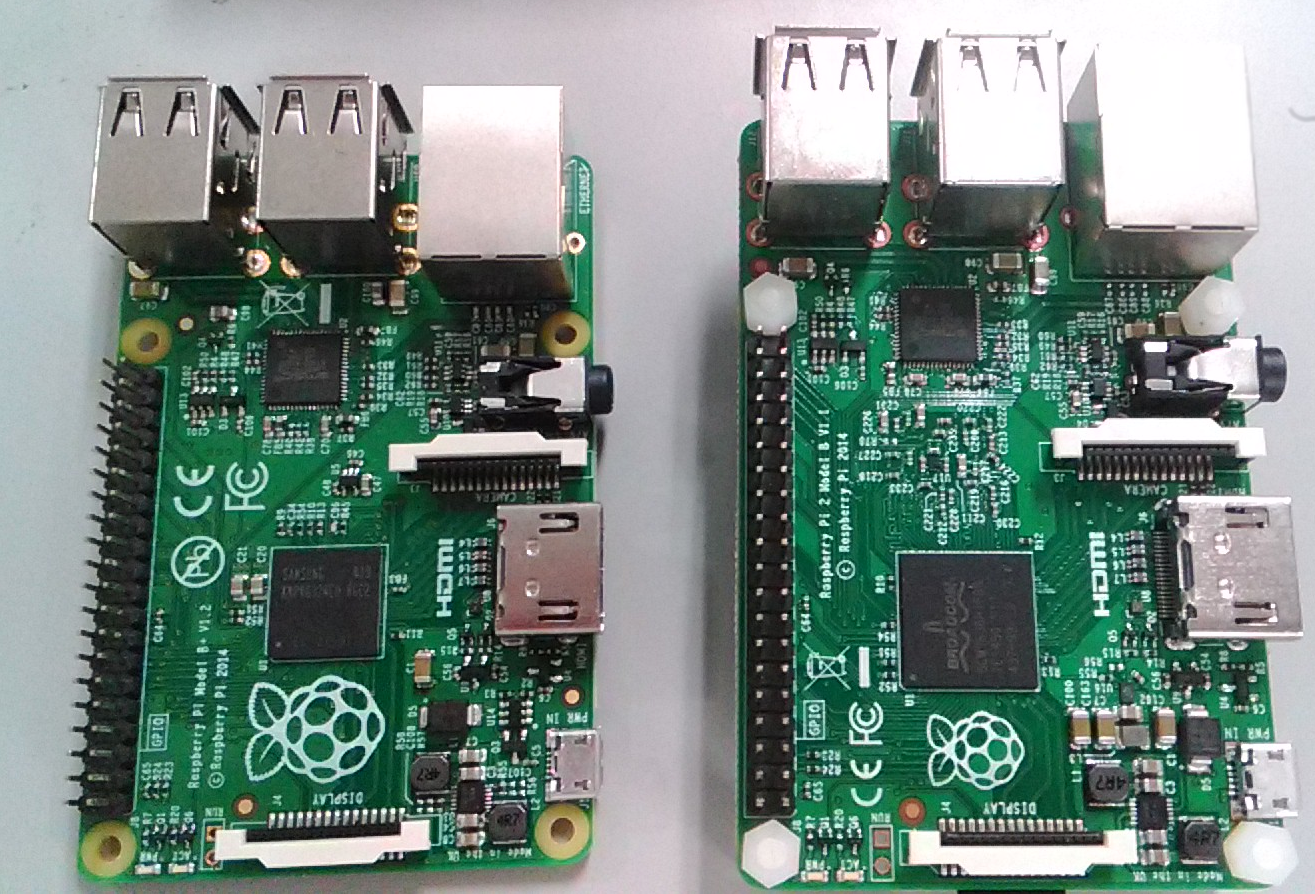
\includegraphics[width=0.7\hsize]{image201503/rpis.png}
\end{center}
\caption{RPi Model B+$B!J:8!K(B $B$H(BRPi 2 Model B$B!J1&!K(B}
\label{fig:rpis}
\end{figure}

RPi (Model B+) $B$H(BRPi 2 Model B $B$N%O!<%I%&%'%"$O(B
$BI=(B\ref{rpi-hw}$B$H$J$j$^$9!#(BCPU$B!"%3%"?t!"%a%b%j$N<oN`$H%5%$%:$,Bg$-$/0[$J$k(B
$B;v$,J,$+$j$^$9!#(BRPi2 $B$G$O%3%"?t$,A}$($F$$$k$?$a!"EE8;$bBg$-$a$N$b$N$,I,MW(B
$B$K$J$C$F$$$k$3$H$bCmL\$9$Y$-E@$G$9!#(B
\begin{table}
\caption{RPi $B$H(BRPi 2 B}
\begin{center}
\begin{tabular}{|c|c|c|}
\hline
-   & RPi Model B+ & RPi 2 Model B \\
\hline
CPU  & ARM1176JZF-S 1$B%3%"(B (700MHz) / ARMv6 & ARM Cortex-A7 4$B%3%"(B (900MHz) / ARMv7\\
SoC  & Broadcom BCM2835 &  Broadcom BCM2836 \\  
CPU  & Broadcom VideoCore IV (250MHz) & $BF1:8(B \\
$B%a%b%j(B & 512MB (SDRAM)& 1GB (LPDDR2 SDRAM) \\
$B%M%C%H%o!<%/(B & LAN9514 (10/100 Mbps) & $BF1:8(B \\
$B30It(BI/O & GPIO 40$B%T%s(B & $BF1:8(B \\
$B%9%H%l!<%8(B & microSD & $BF1:8(B \\
$BEE8;(B & 600 mA (3.0W) & 900 mA (4.5-5.5W) \\
\hline
\end{tabular}
\label{fig:rpi-hw}
\end{center}
\end{table}

Debian armel$B!"(Barmhf$B!"(BRaspbian $B$N0c$$$OI=(B\ref{rpi-sw}$B$NDL$j$G$9!#(B
$B3F%"!<%-%F%/%A%c$G%5%]!<%H$9$kL?Na%;%C%H$,0[$J$j!"(BDebian armel
$B$G$O(B RPi/RPi2 $B$K:GE,2=$5$l$F$$$k$H$O8@$($J$$$3$H$,$o$+$j$^$9!#(B
Unixbench $B$G%Y%s%A%^!<%/$7$?7k2L$rI=(B\ref{rpi-bench}$B$K<($7$^$9!#(B
RPi $B$G$O(B Raspbian $B$N$h$$7k2L$H$J$j!"(BRPi2 $B$G$O(B Debian / armhf $B$,(B
$B$h$$7k2L$H$J$j$^$9!#$3$l$O(B Raspbian $B$,(B ARMv6 / VFPv2 $B$K:GE,2=(B
$B$5$l$?%P%$%J%j$G!"(BRPi2 $B$K:GE,2=$5$l$F$$$J$$$?$a$G$9!#(B
RPi2 $B$G$O(B Raspbian $B$h$j(B Debian / armhf $B$r;H$C$?$[$&$,NI$$$3$H$,(B
$B$o$+$j$^$7$?!#(B

\begin{table}
\caption{Debian $B$H(B Raspbian}
\begin{center}
\begin{tabular}{|c|c|c|c|}
\hline`
 - & Debian armel & Debian armhf & Raspbian \\
\hline
$B%?!<%2%C%HL?Na%;%C%H(B &  ARMv4 & ARMv7 & ARMv6 \\
FPU &  $B$J$7(B &  VFPv3  &  VFPv2 \\
Debian $B%M%$%F%#%V(B & Yes & Yes & No \\
\hline
\end{tabular}
\end{center}
\label{fig:rpi-sw}
\end{table}

\begin{table}
\caption{UnixBench$B$N7k2L(B}
\begin{center}
\begin{tabular}{|c|c|c|c|c|}
\hline`
 - & Debian armel / RPi & Debian armhf /RPi2 & Raspbian / Rpi & Raspbian / Rpi2 \\
\hline
Unixbench (System Benchmarks Index Score) & 66.5 & 450.8 (183.1) & 80.1 & 442.9 (173.8)\\
\hline
\end{tabular}
\end{center}
\label{fig:rpi-sw}
\end{table}


\subsection{Debian armhf / Jessie $B$N%$%s%9%H!<%kJ}K!(B}

$B%$%s%9%H!<%k$K$O(B $B<B5!!"=i4|2=$5$l$F$b$h$$(B4GB$B0J>e$N(BmicroSD$B%+!<%I!"EE8;MQ$N(B
micro USB $B%1!<%V%kEy$,I,MW$G$9!#(B
$B$^$?(BUSB$B%7%j%"%kJQ49%b%8%e!<%k$,$"$k$H%3%s%=!<%k$+$iA`:n$G$-$k$N$G!"%+%9%?%^%$%:(B
$B$,3Z$K$G$-$^$9!#@\B3Nc$r?^(B\ref{fig:rpi2-hw-setting}$B$K<($7$^$9!#(B

\begin{figure}[htbp]
\begin{center}
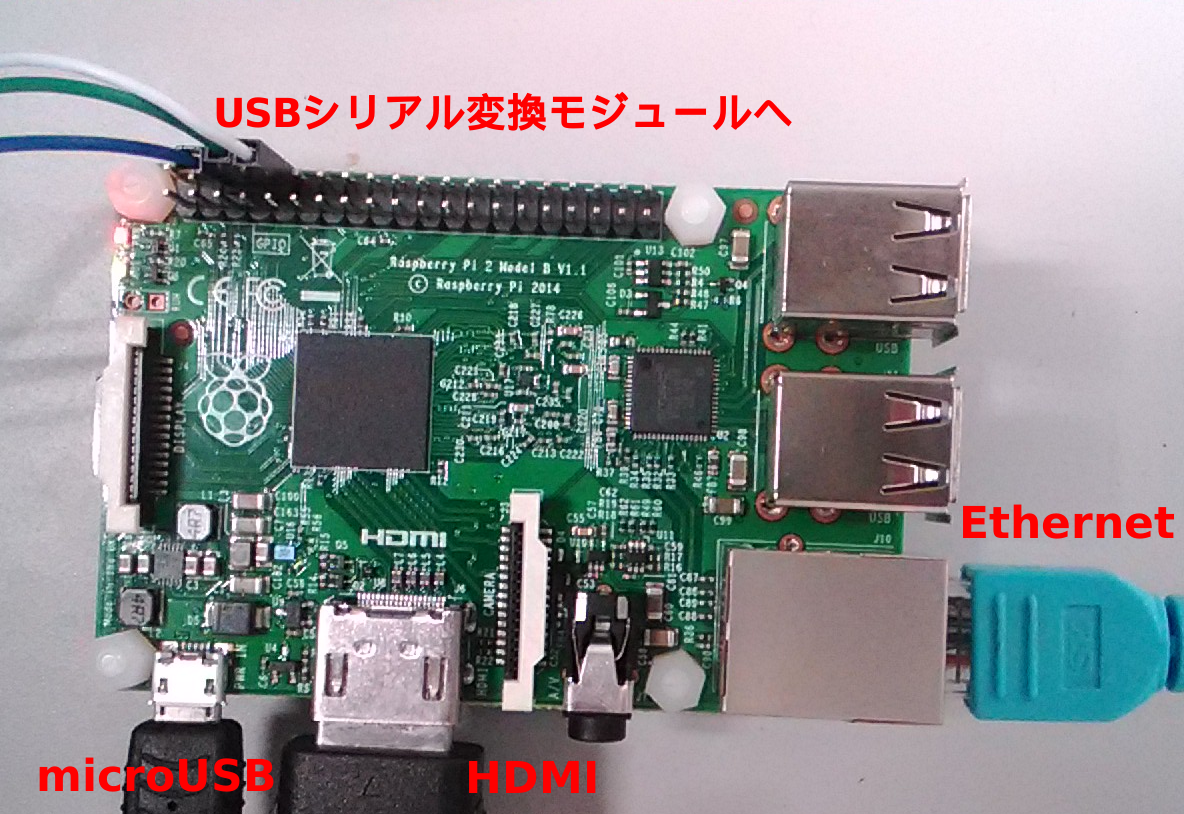
\includegraphics[width=0.7\hsize]{image201503/rpi2-hw-setting.png}
\end{center}
\caption{RPi2 $B@\B3Nc(B}
\label{fig:rpi2-hw-setting}
\end{figure}

$B$^$?%$%s%9%H!<%k$NN.$l$O0J2<$H$J$j$^$9!#(B
\begin{enumerate}
\item microSD$B%+!<%I$NG'<13NG'(B
\item microSD$B%+!<%I$N=i4|2=(B
\item microSD$B%+!<%I$K%Q!<%F%#%7%g%s:n@.(B
\item microSD$B%+!<%I$N%U%)!<%^%C%H(B
\item cdebootstrap $B$r;H$C$F(BmicroSD$B%+!<%I$K%$%s%9%H!<%k(B
\item RPi2$B$N(BLinux$B%+!<%M%k$H%+!<%M%k%b%8%e!<%k$N%$%s%9%H!<%k(B
\item RPi2$B$N%+!<%M%k%3%^%s%I%i%$%s$N@_Dj(B
\item fstab$B$N@_Dj(B
\item $B%M%C%H%o!<%/%G%P%$%9$N@_Dj(B
\item rootfs$BMQ%Q!<%F%#%7%g%s$NJQ99(B
\item root $B$N%Q%9%o!<%I$N@_Dj$H(Brpi$B%f!<%6$NDI2C(B
\item microSD$B%+!<%I$N%"%s%^%&%s%H$H(BRPi2$B$N5/F0(B
\item RPi2 $B$X$N%m%0%$%s(B
\item RPi2 $B@lMQ%D!<%k$N%$%s%9%H!<%k(B
\end{enumerate}

\subsubsection{microSD$B%+!<%I(B $B$N@\B33NG'(B}

$B;HMQ$7$F$$$k(B Debian$B$K(B micorSD $B%+!<%I$rA^F~$7$^$9!#A^F~$9$k$H(Bdmesg$B$K0J2<$N$h$&$J(B
$B%a%C%;!<%8$,=PNO$5$l$k$O$:$G$9!#$3$l$G(BmicroSD$B$,$I$N%G%P%$%9%U%!%$%k$K3d$jEv$F$i$l$?(B
$B$+$o$+$j$^$9!#?^(B\ref{fig:microsd}$B$G$O(B sde $B$K3d$jEv$F$i$l$F$$$k$3$H$,$o$+$j$^$9!#(B

\begin{figure}[htbp]

\begin{commandline}
$ dmesg  | tail -5
[858983.896718] FAT-fs (sdf1): Directory bread(block 32775) failed
[858983.896729] FAT-fs (sdf1): Directory bread(block 1390704) failed
[858983.896731] FAT-fs (sdf1): Directory bread(block 1390705) failed
[869873.800361] sd 6:0:0:3: [sde] 15523840 512-byte logical blocks: (7.94 GB/7.40 GiB)
[869873.831121]  sde: sde1
\end{commandline}
\caption{microSD$B%+!<%I$N%G%P%$%9%U%!%$%k3d$jEv$F3NG'(B}
\label{fig:microsd}
\end{figure}

\subsubsection{microSD$B%+!<%I$N=i4|2=(B}

$B9XF~$7$?$P$+$j$N(BmicroSD$B%+!<%I$O(BVFAT$BEy$G%U%)!<%^%C%H$5$l$F$$$^$9!#(B
MBR$B$,$"$kNN0h$r(B 0 $B$GKd$a$F=i4|2=$7$^$9!J(Bfdisk $B%3%^%s%IEy$GCzG+$K$d$C$F$b$h$$$G$9!K!#(B

\begin{figure}[htbp]
\begin{commandline}
$ sudo dd if=/dev/zero of=/dev/sde bs=1M count=1
\end{commandline}
\caption{microSD$B%+!<%I$N=i4|2=(B}
\label{fig:microsd-format}
\end{figure}

\subsubsection{microSD$B%+!<%I$K%Q!<%F%#%7%g%s:n@.(B}

fdisk $B%3%^%s%I$r;H$C$F(B microSD $B%+!<%I$K%Q!<%F%#%7%g%s$r:n@.$7$^$9!#(B
$B?^(B\ref{fig:createp}$B$K<j=g$r<($7$^$9!#(B
32MB$B!"(BVFAT$B$G(B boot $BMQ$N%Q!<%F%#%7%g%s$r:n@.$7!";D$j$r(Brootfs $BMQ$K(BLinux $BMQ$K:n@.$7$^$9!#(B

$B0l5$$K$d$j$?$$J}$O?^(B\ref{fig:createp2} $B$r<B9T$9$l$P$h$$$G$9!#(B

\begin{figure}[htbp]

\begin{commandline}
$ sudo fdisk /dev/sde
Command (m for help): o

Created a new DOS disklabel with disk identifier 0x9aa4e1fa.

Command (m for help): n
Partition type
   p   primary (0 primary, 0 extended, 4 free)
   e   extended (container for logical partitions)
Select (default p): p
Partition number (1-4, default 1): 1
First sector (2048-15523839, default 2048): 
Last sector, +sectors or +size{K,M,G,T,P} (2048-15523839, default 15523839): +32M

Created a new partition 1 of type 'Linux' and of size 32 MiB.

Command (m for help): t
Selected partition 1
Hex code (type L to list all codes): e
If you have created or modified any DOS 6.x partitions, please see the fdisk documentation for additional information.
Changed type of partition 'Linux' to 'W95 FAT16 (LBA)'.

Command (m for help): n
Partition type
   p   primary (1 primary, 0 extended, 3 free)
   e   extended (container for logical partitions)
Select (default p): p
Partition number (2-4, default 2): 2
First sector (67584-15523839, default 67584): 
Last sector, +sectors or +size{K,M,G,T,P} (67584-15523839, default 15523839): 

Created a new partition 2 of type 'Linux' and of size 7.4 GiB.

Command (m for help): w
The partition figure has been altered.
Calling ioctl() to re-read partition figure.
Syncing disks.
\end{commandline}

\caption{microSD$B%+!<%I$K%Q!<%F%#%7%g%s$r:n@.(B}
\label{fig:createp}
\end{figure}

\begin{figure}[htbp]
\caption{microSD$B%+!<%I$K%Q!<%F%#%7%g%s$r:n@.(B $B0l5$$K$d$k%P!<%8%g%s(B}
\begin{commandline}
(echo o; echo n; echo p; echo 1; echo ; echo +32M; echo t; echo e; echo n; echo p; echo 2; echo ; echo ; echo w) | fdisk /dev/sde
\end{commandline}
\label{fig:createp2}
\end{figure}

\subsubsection{microSD$B%+!<%I$N%U%)!<%^%C%H(B}

$B%Q!<%F%#%7%g%s(B1 $B$O(B mkfs.msdos $B$G!"%Q!<%F%#%7%g%s(B2 $B$O(B mkfs.ext $B$G%U%)!<%^%C%H$7$^$9!#(B
$B%U%)!<%^%C%H$G$-$?$iE,Ev$J%G%#%l%/%H%j$r:n@.$7!"#2$D$N%Q!<%F%#%7%g%s$r%^%&%s%H$7$^$9!#(B
$B:#2s$O(B $B%Q!<%F%#%7%g%s(B1$BMQ$K(B /tmp/boot $B%G%#%l%/%H%j!"%Q!<%F%#%7%g%s(B2$BMQ(B
$B$K(B/tmp/rootfs $B%G%#%l%/%H%j$r:n@.$7!"%^%&%s%H$7$^$9!#(B

\begin{figure}[htbp]
\begin{commandline}
$ sudo mkfs.msdos /dev/sde1
$ sudo mkfs.ext4 /dev/sde2
$ mkdir /tmp/boot /tmp/rootfs
$ sudo mount /dev/sde1 /tmp/boot
$ sudo mount /dev/sde2 /tmp/rootfs
\end{commandline}
\caption{microSD$B%+!<%I$N%U%)!<%^%C%H$H%^%&%s%H(B}
\label{fig:microsdformat}
\end{figure}

\subsubsection{cdebootstrap $B$r;H$C$F(BmicroSD$B%+!<%I$K%$%s%9%H!<%k$9$k(B}

cbootstrap $B$r;H$C$F!"(BmicroSD$B%+!<%I$K(B debian $B5/F0%$%a!<%8$r%$%s%9%H!<%k$7$^$9!#(B
$BA`:n$7$F$$$k%^%7%s$,(BPC$B!J(Bi386$B$d(Bamd64$B!K$N>l9g!"DL>o$O(Barmhf
$B$N%P%$%J%j$r<B9T$G$-$^$;$s!#$=$N$?$a(BPC$BEy$G@h$K%$%s%9%H!<%k$KI,MW$J(BDebian$B%Q%C%1!<%8$N%@%&%s%m!<%I(B
$B$HE83+$r9T$$!"<B:]$N%$%s%9%H!<%k$O(B RPi2 $B$G9T$&$H$$$&J}K!$r<h$j$^$9!#(B
$B<B:]$N%$%s%9%H!<%kJ}K!$O?^(B\ref{fig:firstbootstrap}$B$H$J$j$^$9!#:#2s$N%$%s%9%H!<%k$G$O(B standard $B$G(B
$B;XDj$5$l$F$$$k%Q%C%1!<%8$NB>!"%7%j%"%k%3%s%=!<%k$,;H$($J$$4D6-$r9M$((Bopenssh-server$B!"(B
$B;~4V@_Dj$N$?$a$K(Bntp$B!">ZL@=q$N$?$a$K(Bca-certificates$B!"%(%G%#%?$H$7$F(Bvim$B$r%$%s%9%H!<%k$9$k$h$&$K$7$F(B
$B$$$^$9!#$b$7B>$K0l=o$K%$%s%9%H!<%k$7$?$$%Q%C%1!<%8$,$"$k>l9g$O(B \bf{$-$$-$include}$B$KB3$1$F;XDj$9$k(B
$B;v$,$G$-$^$9!#(B

\begin{figure}[htbp]
\begin{commandline}
$ sudo cdebootstrap --arch=armhf -f standard --foreign jessie \
  --include=openssh-server,ntp,ca-certificates,vim /tmp/rootfs
...
\end{commandline}
\caption{cdebootstrap$B$r;H$C$?(BDebian$B%$%a!<%8$N%$%s%9%H!<%k(B}
\label{fig:firstbootstrap}
\end{figure}

\subsubsection{RPi2$B$N(BLinux$B%+!<%M%k$H%+!<%M%k%b%8%e!<%k$N%$%s%9%H!<%k(B}

$B;DG0$J$3$H$K(BRPi2$B$N(BLinux$B%+!<%M%k$O(BDebian$B$G$ODs6!$5$l$F$$$^$;$s!#$=$NM}M3$H$7$F(B
$B$^$@40A4$K%"%C%W%9%H%j!<%`$G%5%]!<%H$5$l$F$$$J$$;v$H5/F0$K%U%!!<%`%&%'%"$,(B
$BI,MW$H$$$&$3$H$,5s$2$i$l$^$9!#(BDebian$B$G(B RPi2 $B$N(BLinux$B%+!<%M%k$r07$&$K$O(Brpi-update
$B$H$$$&%D!<%k$r;H$&I,MW$,$"$j$^$9!#(B

$B?^(B\ref{fig:kernelinstall}$B$G$O(Brpi-update $B$r(BRPi2 $B$N(Brootfs $B$K%@%&%s%m!<%I$7$?8e!"(B
$B<B9T8"8B$rIU2C$7!"(Brpi-update $B$r;H$C$F%+!<%M%k$H%+!<%M%k%b%8%e!<%k$r%$%s%9%H!<%k$7$^$9!#(B

\begin{figure}[htbp]
\begin{commandline}
$ sudo curl -o /tmp/rootfs/usr/bin/rpi-update https://raw.githubusercontent.com/Hexxeh/rpi-update/master/rpi-update
$ sudo chmod +x /tmp/rootfs/usr/bin/rpi-update
$ sudo mkdir /tmp/rootfs/lib/modules
$ sudo ROOT_PATH=/tmp/rootfs BOOT_PATH=/tmp/boot /tmp/rootfs/usr/bin/rpi-update
*** Raspberry Pi firmware updater by Hexxeh, enhanced by AndrewS and Dom 
 *** Performing self-update
  % Total    % Received % Xferd  Average Speed   Time    Time     Time  Current
                                 Dload  Upload   Total   Spent    Left  Speed
100  8107  100  8107    0     0  54471      0 --:--:-- --:--:-- --:--:-- 54777
 *** Relaunching after update
...
\end{commandline}
\label{fig:kernelinstall}
\caption{rpi-update$B$N%$%s%9%H!<%k$H(BLinux$B%+!<%M%k$N%$%s%9%H!<%k(B}
\end{figure}

\subsubsection{RPi2$B$N%+!<%M%k%3%^%s%I%i%$%s$N@_Dj(B}

RPi2$B$N%+!<%M%k%3%^%s%I%i%$%s$r@_Dj$7$^$9!#(BRPi $B$O(B/boot/cmdline.txt
$B$K5-:\$5$l$F$$$k%+!<%M%k%3%^%s%I%i%$%s$rFI$_9~$s$G5/F0$7$^$9!#(B
$B?^(B\ref{fig:commandlineset}$B$N$h$&$K<B9T$7!"%+!<%M%k%3%^%s%I%i%$%s$r@_Dj$7$^$9!#(B

\begin{figure}[htbp]
\begin{commandline}
$ sudo sh -c "echo dwc_otg.lpm_enable=0 console=ttyAMA0,115200 console=tty1
     root=/dev/mmcblk0p2 rootwait > /tmp/boot/cmdline.txt
\end{commandline}
\label{fig:commandlineset}
\caption{$B%+!<%M%k%3%^%s%I%i%$%s$N@_Dj(B}
\end{figure}

\subsubsection{fstab$B$N@_Dj(B}

fstab$B$N@_Dj$r9T$J$$$^$9!#(Bprocfs$B!"(Brootfs, boot $B%G%#%l%/%H%j$N@_Dj$r5-:\$7$^$9!#(B

\begin{figure}[htbp]
\begin{commandline}
proc            /proc           proc    defaults	0	0
/dev/mmcblk0p1  /boot           vfat    defaults	0	2
/dev/mmcblk0p2  /               ext4    defaults,noatime	0	1
\end{commandline}
\label{fig:rpiconfig}
\caption{fstab$B$N@_Dj(B}
\end{figure}

\subsubsection{$B%M%C%H%o!<%/%G%P%$%9$N@_Dj(B}

rootfs/etc/network/interfaces $B$rJT=8$7!"%M%C%H%o!<%/%G%P%$%9$rM-8z$K$7$^$9!#(B
$B$3$NA`:n$OI,?\$G$O$"$j$^$;$s$,!"(BUSB$B%7%j%"%kJQ49%b%8%e!<%k$r;}$C$F$J$$?M(B
$B$O(BRPi2 $B$K(BSSH$B$G%m%0%$%s$7$FA`:n$9$kI,MW$,$"$j$^$9$N$G!"$3$3$G%M%C%H%o!<%/$r(B
$B5/F0;~$KM-8z$9$k$h$&$K@_Dj$7$F$*$-$^$9!#(B
RPi2 $B$N(BIP$B%"%I%l%9$r(BDHCP$B$+$i<hF@$9$k>l9g$O?^(B\ref{fig:netinterfaces}$B$N$h$&$K@_Dj$7$^$9!#(B

\begin{figure}[htbp]
\begin{commandline}
auto eth0
iface eth0 inet dhcp
\end{commandline}
\label{fig:netinterfaces}
\caption{$B%M%C%H%o!<%/%G%P%$%9$N@_Dj(B}
\end{figure}

\subsubsection{rootfs$BMQ%Q!<%F%#%7%g%s$NJQ99(B}

rootfs/sbin/init $B$K=q$+$l$F$$$k(B 2nd bootstrap $B$NFbMF$K(B
rootfs $B$r%^%&%s%H$9$k9T$,$"$j$^$9!#%G%U%)%k%H$G$O(B rootfs $B$r(B / $B$K%^%&%s%H$9$k(B
$B$h$&5-=R$5$l$F$$$k$?$a!"$3$N$^$^$G$O%$%s%9%H!<%k$K<:GT$7$^$9!#(B
$B@5$7$/%$%s%9%H!<%k$G$-$k$h$&$K(B rootfs $B$r(B /dev/mmcblk0p2 $B$KJQ99$7$^$9!#(B

\begin{figure}[htbp]
\begin{commandline}
trap 'error "Interruped!"' HUP INT TERM

mount -n -o remount,rw rootfs / <- $B$3$l$r(B
mount -n -o remount,rw /dev/mmcblk0p2 / <- $B$3$l$KJQ99(B

chown -hR 0:0 /
\end{commandline}
\label{fig:rpiconfig}
\caption{$B%M%C%H%o!<%/%G%P%$%9$N@_Dj(B}
\end{figure}

\subsubsection{root $B$N%Q%9%o!<%I$N@_Dj$H(Brpi$B%f!<%6$NDI2C(B}

$B8=>u$N$^$^$G$O%$%s%9%H!<%k40N;8e$K%m%0%$%s$G$-$^$;$s!#(B
2nd bootstrap $B;~$K(Broot $B$N%Q%9%o!<%I$r@_Dj$9$k=hM}$rDI2C$7$^$9!#(B
$B$^$?(B rpi$B%f!<%6$r:n@.$7!"%Q%9%o!<%I$r@_Dj$9$k=hM}$bDI2C$7$^$9!#(B
rpi $B%f!<%6$O@bL@$N$?$a$K;H$C$F$$$k$@$1$G$9$N$G!"B>$N%f!<%6L>$G$bLdBj$"$j$^$;$s!#(B

\begin{figure}[htbp]
\begin{commandline}
echo 'deb http://ftp.debian.org/debian jessie main' > /etc/apt/sources.list

echo "root:root" | chpasswd <- $B$3$N9T$rDI2C(B
useradd -m rpi <- $B$3$N9T$rDI2C(B
echo rpi:rpi | chpasswd <- $B$3$N9T$rDI2C(B

run rm /sbin/init
\end{commandline}
\label{fig:rpiconfig}
\caption{root $B%Q%9%o!<%I$N@_Dj(B}
\end{figure}

\subsubsection{microSD$B%+!<%I$N%"%s%^%&%s%H$H(BRPi2$B$N5/F0(B}

microSD$B%+!<%I$r%"%s%^%&%s%H$7!"(BPRi2 $B$N(B microSD$B%+!<%I%9%m%C%H(B
$B$KA^F~$7$^$9!#A^F~8e!"(Bmicro USB $B%1!<%V%k$r(B RPi2 $B$KA^$7!"(B
RPi2$B$r5/F0$7$^$9!#5/F0$9$k$H<+F0E*$K(B2nd bootstrap $B$,<B9T$5$l!"(B
RPi2$B>e$G%$%s%9%H!<%k$,<B9T$5$l$^$9!#(B
$B$b$7(BHDMI$B@\B3$,$G$-$k%b%K%?!<$r;}$C$F$$$k>l9g$O!"(BRPi2 $B$H@\B3$9$k$H(B
$B%$%s%9%H!<%k$5$l$kMM;R$r3NG'$G$-$^$9!#(B
$B%$%s%9%H!<%k40N;$^$G#3#0J,$[$IBT$?$5$l$k$N$G!"5$D9$KBT$A$^$7$g$&!#(B
HDMI$B$,MxMQ$G$-$k%b%K%?!<$r;}$C$F$J$$>l9g!"%$%s%9%H!<%k$,40N;$7$?$+(B
$B8+$?L\$G$O$o$+$i$J$$$N$G!"(BRPi2 $B$K(BIP$B%"%I%l%9$,3d$jEv$F$i$l$F$$$k$+!"(Bping $B$r(B
$B<B9T$7$FH?1~$,$"$k$+$J$I$G3NG'$9$kI,MW$,$"$j$^$9!#(B

\subsubsection{RPi2 $B$X$N%m%0%$%s(B}

$B%$%s%9%H!<%k$,40N;$9$k$H<+F0E*$K(B init $B$,:F<B9T$5$l!"(BDebian $B$,N)$A>e$,$C$?>uBV$K$J$C$F$$$^$9!#(B
USB$B%7%j%"%k%b%8%e!<%k7PM3$d!"(BSSH$B7PM3$G%m%0%$%s$G$-$k$h$&$K$J$C$F$$$^$9$N$G!"%m%0%$%s$7$F(B
$B$/$@$5$$!#8e$ODL>o$N(BDebian$B$HJQ$o$j$^$;$s!#(B

\subsubsection{RPi2 $B@lMQ%D!<%k$N%$%s%9%H!<%k(B}

RPi2 $B$N@lMQ%D!<%k$G$"$k(B rpi-update$B!"(Braspi-config $B$O$^$@(BDebian$B$G$ODs6!$5$l$F$$$^$;$s!#(B
$B$3$l$i$O%+!<%M%k$d%U%!!<%`%&%'%"$N%"%C%W%G!<%H!"(BRPi$B%O!<%I%&%'%"$N@_Dj$r9T$&$?$a$N5!G=$,(B
$BEk:\$5$l$F$*$j!"(BRPi $B%f!<%6$K$OI,?\$N%D!<%k$H$J$C$F$$$^$9!#(B
$B$3$l$r(B Debian $B$GMxMQ$G$-$k$h$&$K$9$k$K$O(B raspberrypi.org $B$GDs6!$5$l$F$$$k(B $B3F%D!<%k$N(B
Debian $B%Q%C%1!<%8$r%$%s%9%H!<%k$9$kI,MW$,$"$j$^$9!#(B
$B?^(B\ref{fig:rpirep}$B$K@_DjJ}K!$r<($7$^$9!#(B

\begin{figure}[htbp]
\begin{commandline}
# wget -O - http://archive.raspberrypi.org/debian/raspberrypi.gpg.key | apt-key add - 
# echo deb http://archive.raspberrypi.org/debian wheezy main >> /etc/apt/sources.list
# apt-get update
# apt-get install rpi-update raspi-config
\end{commandline}
\label{fig:rpirep}
\caption{rpi-config$B!"(Brpi-update $B%Q%C%1!<%8$N%$%s%9%H!<%kJ}K!(B}
\end{figure}

\subsubsection{$B=*$o$j$K(B}

RPi2 $B$+$i(B $B%M%$%F%#%V$N(BDebian$B$,MxMQ$G$-$k$h$&$K$J$j$^$7$?!#(B
$B%$%s%9%H!<%i$d(BmicroSD$B%+!<%I%$%a!<%8$,=`Hw$5$l$F$$$J$/$F$b!":#2s2r@b$7$?J}K!$r;H$&$H(B
RPi2 $B$K<+J,9%$_$N(BDebian$B$r%$%s%9%H!<%k$G$-$k$h$&$K$J$j$^$9!#(BCPU$B$b6/2=$5$l$=$3$=$3;H$$(B
$B$d$9$/$J$C$?(B Rpi2 $B$G(B Debian$B$r?($C$F$_$F$O$$$+$,$G$7$g$&$+!#(B

\cleartooddpage

\vspace*{15cm}
\hrule
\vspace{2mm}

\includegraphics[width=2cm]{image200502/openlogo-nd.eps}
\noindent \Large \bf Debian $BJY6/2q;qNA(B\\
\noindent \normalfont \debmtgyear{}$BG/(B\debmtgmonth{}$B7n(B\debmtgdate{}$BF|(B \hspace{5mm}  $B=iHGBh(B1$B:~H/9T(B\\
\noindent \normalfont $BEl5~%(%j%"(B Debian $BJY6/2q(B $B!JJT=8!&0u:~!&H/9T!K(B\\
\hrule

\end{document}
